\subsection{CSCW y Sistemas Groupware}
El trabajo colaborativo tiene un alto impacto hoy en d\'ia, ya que las personas pueden realizar m\'as r\'apido una tarea compleja si tienen los elementos necesarios para poder llevar a cabo una colaboraci\'on eficiente, hay muchas formas de trabajo colaborativo, y el contexto en el que se desarrolla es muy diverso. El \'area de CSCW se concentra en las actividades colaborativas, y el hecho de que m\'ultiples individuos situados en diferentes escenarios de trabajo y situaciones, con diferentes responsabilidades, perspectivas y propensiones interact\'uen sean mutuamente dependientes en el conducto de su trabajo tienen implicaciones importantes en el dise\'no de sistemas computacionales dirigidos a apoyar estos esfuerzos \cite{schmidt1992taking}.

Shmidt et al. menciona un conjunto de caracter\'isticas que se deben de tomar en cuenta para que los sistemas computacionales que estudia el CSCW sean aceptables para los usuarios \cite{schmidt1992taking}:
\begin{itemize}
\item Las unidades cooperativas son grandes o son parte de conjuntos m\'as grandes.
\item Las unidades cooperativas son, por lo general, formaciones de poca duraci\'on, emergen para manejar una situaci\'on particular y luego se disuelven.
\item La afiliaci\'on de las unidades cooperativas no son estables y normalmente no determinable. Las unidades cooperativas a veces se intersectan.
\item El patr\'on de interacci\'on en trabajos cooperativos cambia din\'amicamente con los requerimientos y restricciones de la situaci\'on.
\item El trabajo cooperativo es distribuido f\'isicamente en tiempo y espacio.
\item El trabajo cooperativo es distribuido l\'ogicamente, en t\'erminos de control, es decir, los agentes son semi-aut\'onomos en su trabajo parcial.
\item El trabajo cooperativo involucra perspectivas inconmensurables (e.g. profesiones, especialidades, funciones de trabajo, responsabilidades, etc.) as\'i como estrategias incongruentes y motivos discordantes.
\item No hay agentes omniscientes en el trabajo cooperativo en escenarios naturales.
\end{itemize}
\subsection{Groupware}
Como ya se mencion\'o anteriormente los groupware son sistemas que apoyan el trabajo colaborativo de un grupo de personas, y lo hace brindando comunicaci\'on e informaci\'on relevante al usuario. Una de las taxonom\'ias cl\'asicas de groupware es la de Johansen \cite{johansen1988groupware} quien propone 2 dimensiones de los groupware: tiempo y espacio.

\begin{figure}[h!]
  \centering
  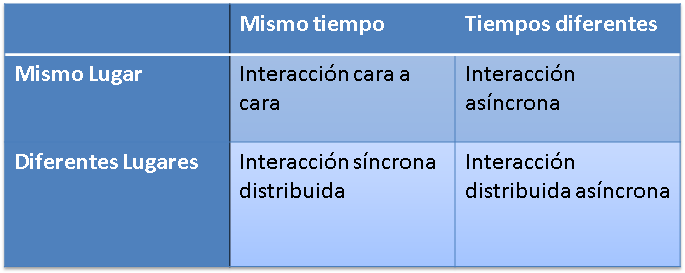
\includegraphics[scale=0.6]{dimen}
  \caption{Dimensiones de los groupware por tiempo y espacio \cite{johansen1988groupware}}
\end{figure}

En un estudio m\'as reciente realizado por Cruz \cite{cruz2012towards} hace una recopilaci\'on de los atributos pertenecientes a un groupware, que son din\'amicas de trabajo en escenarios de colaboraci\'on (comunicaci\'on, cooperaci\'on, y coordinaci\'on), dimensiones temporales y espaciales, caracter\'isticas grupales (tipos de tareas grupales, caracter\'isticas y tama\'no), categor\'ias t\'ecnicas de aplicaciones groupware (escalabilidad, software y hardware), y categor\'ias complementarias (e.g. usabilidad). A partir de estos atributos propone un modelo socio-t\'ecnico de clasificaci\'on para groupwares.

\begin{figure}[h!]
  \centering
  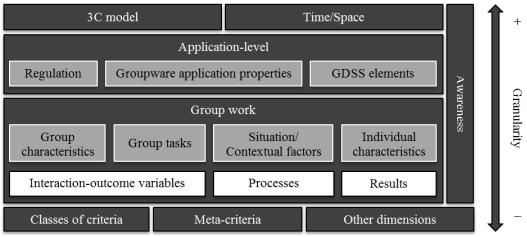
\includegraphics[scale=0.9]{socclass}
  \caption{Modelo socio t\'ecnico de clasificaci\'on de groupware seg\'un Cruz \cite{cruz2012towards}}
\end{figure}

En la primera categor\'ia se encuentra el modelo 3C, que se enfoca en la comunicaci\'on, la coordinaci\'on y la cooperaci\'on.  Algunas categor\'ias de relacionadas a la coordinaci\'on en la literatura revista por Cruz \cite{cruz2012towards} son: planeaci\'on, modelos de control, relaciones entre tareas y subtareas, y manejo de la informaci\'on, ajuste mutuo, estandarizaci\'on, protocolos de coordinaci\'on, manejo temporal, recursos, o artefactos compartidos producidos durante la sucesi\'on de actividades. Entre las categor\'ias de cooperaci\'on se pueden encontrar desde producci\'on (co-autor\'ia), almacenamiento o manipulaci\'on de artefactos, hasta concurrencia, control de acceso.

Otro aspecto que toma Cruz en su modelo (figura anterior) es tiempo y espacio de donde se observan las siguientes subcategor\'ias: persistencia de sesi\'on, retardo en transmisi\'on de audio/video, reciprocidad y homogeneidad de canales, retardo de env\'io de mensajes, y espontaneidad de colaboraci\'on. En la categor\'ia de nivel de aplicaci\'on se identifican tipolog\'ias que clasifican a los groupware de acuerdo a su enfoque en el nivel del grupo. Como subcategor\'ia se encuentran la regulaci\'on, que son los mecanismos que permiten a los participantes organizarse en un ambiente compartido; en la literatura algunas de las dimensiones de regulaci\'on que se encuentran son: arenas(ubicaci\'on); actores(roles, lugares, y posiciones); herramientas(regulativas o no); roles(tem\'aticos o casuales); reglas(restricciones, normas o reglas de trabajo); tipos de interacci\'on; escenarios interactivos; y objetos(medios de comunicaci\'on y productos de colaboraci\'on). Otra subcategor\'ia del nivel de aplicaci\'on son las propiedades de la aplicaci\'on groupware entre las que se pueden encontrar arquitectura, cualidades funcionales y de calidad, soporte para procesos grupales, interfaz de colaboraci\'on(portales, dispositivos o espacio de trabajo f\'isico), relaciones(colecciones, listas, \'arboles y gr\'aficas), funciones de n\'ucleo, contenido(texto, ligas, gr\'aficas o flujo de datos), acciones soportadas(recibir, agregar, asociar, editar, mover, borrar, o juzgar), identificaci\'on, controles de acceso, mecanismos de alerta, componentes inteligentes, indicadores de consciencia, y plataforma, los elementos GDSS incluyen hardware, software y soporte de personas.

La siguiente capa del modelo se enfoca a los grupos, los cuales son definidos como una \"agregaci\'on social de individuos\" con consciencia de su presencia, conducida por sus propias normas, y soportado por interdependencias de tareas hacia una meta en com\'un en un contexto compartido \cite{pumareja2002evolutionary}. Dentro de esta categor\'ia se encuentran las subcategor\'ias: tareas grupales, caracter\'isticas del grupo, factores de situaci\'on, y caracter\'isticas individuales.

Un groupware se puede caracterizar por 3 aspectos complementarios importantes desde la vista del usuario: una descripci\'on de los objetos y las operaciones que se pueden hacer sobre ellos y que est\'an disponibles para los usuarios, una descripci\'on de los aspectos din\'amicos del sistema (flujo de control y  de datos) y una descripci\'on de la interfaz entre el sistema y los usuarios y entre los usuarios \cite{ellis1994conceptual}. Este modelo es llamado de coordinaci\'on y describe la organizaci\'on de las actividades realizadas por los usuarios y no por el sistema. Los componentes principales de este modelo ontol\'ogico son los objetos y las operaciones. Las operaciones sobre objetos son aspectos importantes que determinan el nivel de contribuci\'on de un usuario al trabajo\cite{ellis1994conceptual}, e.g. en un sistema editor de c\'odigo colaborativo, los usuarios que realicen m\'as operaciones sobre un archivo(actualizar el archivo, crear archivo, eliminar archivo) son los que m\'as aportan al proyecto, sin embargo la desventaja de esto es que no se sabe si la operaci\'on que se hizo produjo resultados positivos, as\'i un usuario que realice varios cambios sobre un archivo puede ser se\'nal de que se equivoca mucho en su redacci\'on, otros aspectos importantes en la colaboraci\'on son la interacci\'on con miembros del grupo y el ambiente para resolver problemas, tomar decisiones, mantener la afiliaci\'on del grupo, etc.

Antunes\cite{antunes2008structuring} presenta un framework detallado para evaluar los sistemas colaborativos bajo desarrollo de acuerdo a variables dadas y niveles de desempe\'no. Considera dos dimensiones: una define el conjunto de variables de evaluaci\'on relevantes y el otro se ocupa de los niveles de desempe\'no que los usuarios evaluados. El tiempo de evaluaci\'on es inherentemente asociado con el proceso de desarrollo. Menciona una lista de m\'etodos de evaluaci\'on de groupwares son: 

\begin{itemize}
\item Evaluaci\'on heur\'istica de Groupware:(Backer et al 2002) es basado en ocho heur\'isticas groupware como una lista de caracter\'isticas que los groupware deber\'ian de tener. Los problemas que surjan se apuntan y se corrigen.
\item Groupware walkthrough: (Pinelle and Gutwin 2002) un escenario es una descripci\'on de una actividad o conjunto de actividades, que incluye a los usuarios, su conocimiento, el resultado esperado y las circunstancias que los rodean.
\item Collaboration Usability Analisys (Pinelle et al. 2003): los evaluadores mapean acciones colaborativas a un conjunto de mecanismos de colaboraci\'on, o representaciones granulares de acciones colaborativas b\'asicas, que pueden estar relacionadas con elementos en la interfaz de usuario, los diagramas resultantes capturan detalles sobre componentes de tareas, una noci\'on del flujo a trav\'es de ellos y la distribuci\'on de tareas.
\item Groupware Observational User Testing (Gutwin and Greenberg 2000) los evaluadores observan como los usuarios realizan actividades particulares soportadas por un sistema en un ambiente controlado. Los evaluadores monitorean a los usuarios que tienen problemas con una tarea, o piden a los usuarios pensar en voz alta sobre lo que est\'an realizando
\item Human-Performance Model (Antunes et al. 2006): los evaluadores descomponen las interfaces en espacios de trabajo compartidos, definen escenarios cr\'iticos enfocados a acciones colaborativas para los espacios compartidos y comparan el desempe\'no del grupo en escenarios cr\'iticos para predecir tiempos de ejecuci\'on.
\item Enfoque de Manejo de conocimiento (Vizca\'ino et al. 2005): se mide si el sistema ayuda a los usuarios a detectar flujos de conocimiento y diseminar, reusar y almacenar conocimiento. El proceso de circulaci\'on de movimiento se comprende de 6 fases (creaci\'on de conocimiento, acumulaci\'on, divisi\'on, utilizaci\'on, internalizaci\'on), la evaluaci\'on se realiza contestando preguntas relacionadas a cada \'area.
\end{itemize}

Adem\'as de estos aspectos inherentes al trabajo colaborativo, es importante que los groupware proporcionen a los usuarios medios con los que puedan articular el trabajo que est\'an realizando de manera grupal, estos medios deben de apoyar la comunicaci\'on, la coordinaci\'on y la cooperaci\'on de los miembros del grupo. Para que esto se logre con mayor naturalidad es necesario mantenerlos al tanto de la situaci\'on del grupo, el estado de las actividades que se est\'an realizando, el objetivo que persigue el grupo, etc. a esto se le llama consciencia.

La consciencia se refiere al conocimiento que tienen los individuos sobre s\'i mismos y sobre el ambiente que los rodea, y en el caso de trabajo colaborativo, el rol que desempe\'nan en su grupo y el estado de los dem\'as integrantes.

Para que pueda haber cooperaci\'on, los miembros de un grupo deben estar consciencia de las actividades que realizan los dem\'as, creando consciencia del grupo en el espacio de trabajo \cite{cruz2012towards}. El ciclo de colaboraci\'on est\'a limitado por la consciencia, que es la percepci\'on del grupo acerca de lo que cada miembro desarrolla, y el conocimiento contextual que tienen sobre qu\'e est\'a pasando entre el grupo \cite{mittleman2008toward}. Cruz \cite{cruz2012towards} caracteriza awareness por:
\begin{itemize}
\item consciencia espacial y atmosf\'erica
\item consciencia de la actividad
\item consciencia de los objetos
\item consciencia humana
\item consciencia presencial
\item consciencia influencial
\item consciencia de habilidades
\item consciencia contextual
\end{itemize}

\subsection{Consciencia contextual}
Consciencia contextual es el entendimiento de las actividades de los dem\'as usuarios, que proporciona un contexto para las actividades propias \cite{dourish1992awareness}. El problema de mantener la consciencia del espacio de trabajo en los groupware gira en torno a la obtenci\'on de informaci\'on \'util m\'as que el c\'omo la utilizan los usuarios \cite{ardissono2012context}. La informaci\'on a ser recabada se ocupa de qui\'en est\'a trabajando en un contexto compartido, qu\'e est\'an haciendo, d\'onde est\'an trabajando, cu\'ando ocurren varios eventos, y como suceden esos eventos \cite{ardissono2012context}. Similar a las interacciones cooperativas entre un grupo de personas, la consciencia contextual aumenta la experiencia que un individuo tiene en cualquier escenario de asistencia, el manejo de acoplamiento de actividades, la coordinaci\'on de acciones cooperativas, anticipaci\'on de actividades humanas o ambientales tanto como futuras intenciones, y la b\'usqueda de ayuda son aspectos b\'asicos de una interacci\'on que puede ser mejorada mediante la consciencia contextual \cite{aehnelt2012discussion}.
\subsection{C\'omputo Consciente del Contexto}
\subsubsection{Contexto}
Contexto es tradicionalmente la localizaci\'on, identidad, y estado de las personas, grupos y objetos virtuales y f\'isicos. seg\'un pereira \cite{pereira2013CSCWD} el contexto puede ser visto como un conjunto de condiciones e influencias en una situaci\'on relevante y que la hacen \'unica y comprensible, esta situaci\'on puede referirse a una persona, grupo de personas, objeto f\'isico, entidad computacional, etc. El concepto de modelos mentales tiene una relaci\'on muy cercana a la consciencia contextual y situacional \cite{aehnelt2012discussion}, al momento de modelar contexto, es necesario distinguir entre los diferentes tipos de informaci\'on contextual\cite{hoyos2013domain}, el contexto de las actividades colaborativas pueden ir desde un editor de documentos distribuido, hasta un videojuego de primera persona; por lo que los elementos particulares de dichas actividades cambia muy radicalmente de uno a otro, y con esto surge la necesidad de usar una taxonom\'ia con un alto nivel de abstracci\'on que soporte la diversidad de contexto con los que se trabaja.

En una revisi\'on de la literatura sobre modelos contextuales se revisaron ontolog\'ias contextuales, entre las que se pod\'ian encontrar los siguientes elementos:

\begin{center}
\begin{longtable}{|p{3cm}|p{10cm}|}
\caption{Unidades contextuales encontradas en los frameworks revisados.}\\
\hline
\textbf{Elementos} & \textbf{Descripci\'on}\\
\hline
\endfirsthead
\multicolumn{2}{c}%
{\tablename\ \thetable\ -- \textit{Contin\'ua de p\'agina anterior}} \\
\hline
\textbf{Elementos} & \textbf{Descripci\'on} \\
\hline
\endhead
\hline \multicolumn{2}{r}{\textit{Contin\'ua en siguiente p\'agina}} \\
\endfoot
\hline
\endlastfoot

	Objetos o artefactos & Entidades sobre las que los usuarios pueden realizar alguna acci\'on. \\
	\hline
	Tareas & Acciones asociadas con usuarios, objetos, objetivos y subtareas que se deben de llevar a cabo para alcanzar un objetivo. \\
	\hline
	Eventos & Eventos ocurridos en interacciones\cite{montane2013context}\\
	\hline
	Usuarios & Entidades que pertenecen a una comunidad y que realizan tareas\cite{montane2013context}. \\
	\hline
	Ubicaciones & Posici\'on virtual o f\'isica en un grupo \cite{montane2013context}. \\
	\hline
	Grupos & Colecci\'on de usuarios que realizan una actividad\cite{montane2013context}. \\
	\hline
	Objetivos & Los objetivos de la comunidad\cite{montane2013context}. \\
	\hline
	Alianzas & Subconjunto de usuarios en un grupo \cite{montane2013context}. \\
	\hline
	Actividades & Actividades realizadas por un grupo\cite{montane2013context}. \\
	\hline
	Reglas & Comportamientos definidos por el grupo \cite{montane2013context}. \\
	\hline
	Foco de visi\'on & D\'onde est\'an mirando los usuarios\cite{gallardo2012framework}. \\
	\hline
	Vistas de sistema, espacios de trabajo & Qu\'e pueden ver los usuarios \cite{gallardo2012framework}. \\
	\hline
	Alcance & Alcance de los usuarios\cite{gallardo2012framework}. \\
	\hline
	Presencia & Presencia de usuarios en el espacio de trabajo\cite{gallardo2012framework}. \\
	\hline
	Intenci\'on & De qu\'e objetivo es parte una tarea\cite{gallardo2012framework}. \\
	\hline
	Habilidades & Capacidad para llevar a cabo un conjunto de actividades con cierto nivel de destreza \cite{decouchant2013adapting}. \\
	\hline
	Contexto f\'isico & Incluye todas las magnitudes f\'isicas (e.g. tiempo, espacio, temperatura, nivel de luz, nivel de ruido)\cite{hoyos2013domain}. \\
	\hline
	Contexto computacional & Informaci\'on relacionada con el software y hardware de sistemas, e.g. trafico de red, condiciones, estatus de hardware, informaci\'on pedida por el usuario, requerimientos de memoria\cite{hoyos2013domain}. \\
	\hline
	Ambiente & Descripci\'on de la distribuci\'on f\'isica de los objetos y usuarios en un espacio de trabajo\cite{hoyos2013domain}. \\
	\hline
\end{longtable}
\end{center}

Todos estos elementos se extrajeron de diferentes modelos entre los que se hizo la siguiente tabla comparativa:

\begin{figure}[h!]
  \centering
    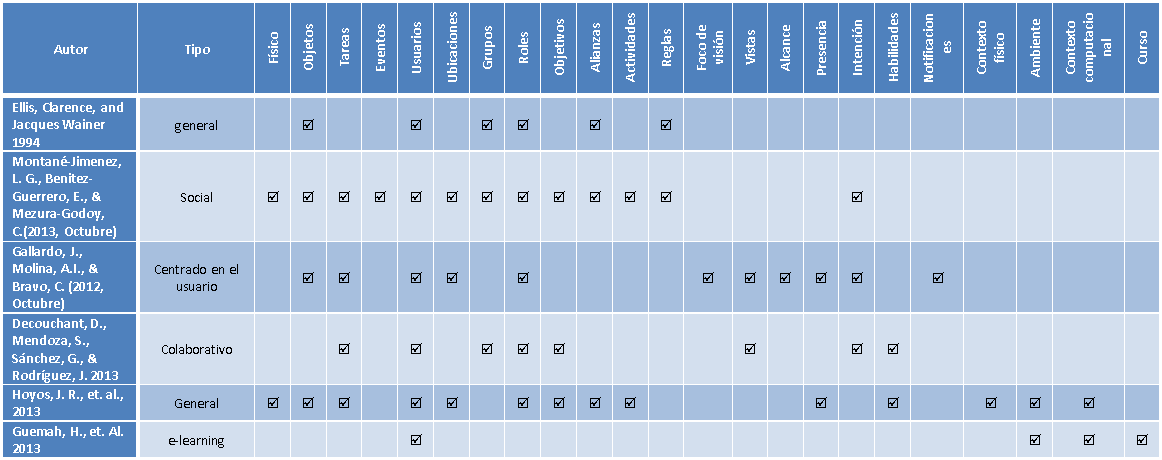
\includegraphics[scale=0.7]{cmpcntx}
  \caption{Comparaci\'on de modelos de contexto\cite{ellis1994conceptual}\cite{montane2013context}\cite{gallardo2012framework}}
\end{figure}

Alves hace tres definiciones clave para el modelado de contexto y para su propagaci\'on \cite{alves2013radiator}, la primera es una definici\'on de contexto: Un atributo $A_{i}$ es una tupla $( N, V )$, donde \textit{N} es un nombre representando el atributo(por ejemplo, velocidad) y $V$ es el valor del atributo(e.g., 100); $P$ es un conjunto finito de personas ${P_{1},P_{2}...P_{n}}$; $t$ es el rango de tiempo entre dos marcas de tiempo; y $\textit{A}$ un conjunto finito de atributos ${A_{1},A_{2}...A_{n}}$.

Contexto \textit{C} es una 3-tupla $( P, t, A )$ que representa los atributos que caracteriza la situaci\'on de un grupo de personas $P$ durante un intervalo de tiempo $t$. Por ejemplo suponiendo que Alice est\'a en Nueva York entre Julio 1 y Julio 3. Podemos definir su contexto $C$ como:

$C=( ( Alice ), 01/07..03/07, ( Ubicacion, Nueva York ))$

La segunda definici\'on es de agregaci\'on, sugerida para reducir la cantidad de informaci\'on a procesar y reducir la carga de red, define agregaci\'on como ${ ( P_{1},t_{1},A_{1} ),..., ( P_{n},t_{n},A_{n} ) }$ es un conjunto de contextos y $Ac$ un atributo en com\'un tal que para todo atributo $A_{i}$ perteneciente a $A_{1} ... A_{n}$, $Ac$ pertenece a $A_{i}$.

$Aggr( A_{c}, {( P_{1},t_{1},A_{1} ),..., ( P_{n},t_{n},A_{n} )}) = ( P, t, A )\Rightarrow \forall P_{i}\in P_{1}...P_{n}:P_{i}\in P \wedge \forall t_{i} \in t_{1}...t_{n}:t_{i}\subseteq t \wedge \forall A_{i}\in A_{1}...A_{n}:A_{i}\in A$

Por \'ultimo as\'i define agregabilidad, $CP$ es el contexto actual de una persona $P$ y $C_{x}$ el contexto de alguien m\'as que el sistema quiere propagar a $P$.

La funci\'on de Agregabilidad $G( CP, C_{x} )$ representa que tan agregado debe de estar $C_{x}$ antes de ser transmitido a $P$ , tomando en consideraci\'on el contexto actual de $CP$.

Por lo tanto un conjunto de contextos $C_{1}..C_{n}$ es solo propagado a $P$ cuando para todo $i$ perteneciente a $1..n$, $G( CP, C_{i} ) = n$, $n$ siendo un entero. Informalmente la agregabilidad representa el n\'umero de mensajes de contexto que deben de ser retenidos antes de su propagaci\'on, si se define una funci\'on $G$ que siempre regrese 4, el sistema siempre va a agregar cuatro mensajes contextuales antes de propagarlos"

En el trabajo de Ardissono \cite{ardissono2012context} mencionan activity frames para simplificar el contexto de actividades cooperativas, un frame era definido por una 5-tupla $( fn, U, O, Oi, T )$, donde $fn$ era el nombre del frame, $U$ el conjunto de usuarios involucrados en la actividad, $O$ los objetos asociados al frame, $Oi$ es el conjunto de objetos del frame por medio de inferencias, y $T$ las tareas asociadas a la actividad. Y a su vez las tareas est\'an formadas por $( tn, U, O, Oi, g, P, T, s, d )$, donde $tn$ es el nombre de la tarea, $U$, $O$ y $Oi$ como dicho antes son los Usuarios, Objetos, y objetos inferidos asociados a la tarea, $g$ es el objetivo, $P$ es el grupo de tareas que deben de estar cerradas antes de iniciar $tn$, $T$ es el conjunto de tareas hijas, $s$ es el estado(habilitada, deshabilitada, cerrada) y $d$ es la fecha l\'imite para terminar la tarea, nula por defecto.

En el a\~no 2013 se propone MARS que es un modelo contextual de regulaci\'on y lenguaje asociado, ayuda a modelar la actividad soportada por herramientas groupware. En este modelo las interacciones toman lugar en un espacio llamado arena, cada interacci\'on es representada por un escenario que describe la forma en que se lleva a cabo dicha interacci\'on, qui\'enes participan y los objetos involucrados, adem\'as se definen condiciones y precondiciones para que este escenario se lleve a cabo; en esta arena est\'an presentes actores que realizan acciones, durante esta actividad se manejan o producen objetos; actores y objetos pertenecen a diferentes familias y desempe\'nan diferentes papeles o roles. Dado que los miembros de un grupo colaborativo pueden serlo a su vez de otro, se definen vistas que determinan los actores, objetos e interacciones que una arena puede compartir con otra.

Junto con MARS viene un lenguaje de regulaci\'on para describir escenarios llamado CORAL\footnote{Collaborative Regulation Language} que toma en cuenta tres aspectos de los escenarios definidos en MARS especificados en las pre y pos condiciones de la interacci\'on: quién puede participar en la interacci\'on, qu\'e objetos pueden ser manipulados, qu\'e rol tiene un actor u objeto durante la interacci\'on y en casos similares, referencias a otros escenarios. Con esto se define el lenguaje CoRaL con la siguiente sintaxis descrita en noteaci\'on BNF. Siendo E el conjunto de elementos de cadenas de nombres de arenas, actores, familias de actores, familias de objetos, objetos y roles:
	
\begin{gather}
	Aqui va el lenguaje
		
   <sentencia> $::=$ <expresión><operador><expresión>";"
       
    <expresion> $::=$ <palabraReservada>:${$<elementos>$}$
    
    <expresion> $::=$ $!<$palabraReservada$>:{$<elementos>$}$
    
    <operador> $::= :: | ->$
    
    <palabraReservada> $::=$ "Arena" | "Interaccion" | "Actor" | "Familia de actor" | "Familia de Objeto" | "Objeto" | "Rol"
    
    <elemento> $::=$ cualquier cadena en E    
\end{gather}

Un modelo enfocado en el contexto social de aplicaciones groupware clasifica los elementos contextuales en 3 categor\'ias: la interactiva, la cohesiva y la afectiva \cite{montane2013context}. En la interactiva se encuentran variables como: objetos, tareas, eventos, usuarios, y ubicaciones; en la cohesiva se pueden observar a grupos, roles, objetivos, alianzas, actividades, y reglas; por \'ultimo est\'an las variables afectivas en las que se encuentran las emociones y los gestos de los usuarios.	

\subsubsection{Proceso}

Para obtener resultados de un conjunto de variables contextuales se establecen 3 pasos ya descritos antes \cite{montane2013context}: recuperar las variables contextuales en un formato legible para la computadora, almacenar, recuperar y actualizar los datos contextuales de una base de datos, e inferir resultados de un conjunto particular de variables asociadas unas con otras.

\subsubsection {Adquisici\'on de contexto}
 Antunes propone un marco de trabajo para evaluar groupwares \cite{antunes2008structuring}, un enfoque entrada-procesamiento-salida para conceptualizar las relaciones entre el soporte tecnol\'ogico y factores relacionados al comportamiento del grupo y contexto de trabajo. Las variables contextuales son factores importantes para describir el comportamiento del grupo, est\'an clasificadas en 5 categor\'ias generales \cite{antunes2008structuring}: personales, situacionales, estructura del grupo, caracter\'isticas de la actividad o tarea y caracter\'isticas tecnol\'ogicas. Los procesos grupales est\'an definidas como las caracter\'isticas de las interacciones del grupo, incluyendo las decisionales, comunicacionales, e interpersonales. Por \'ultimo este framework eval\'ua los resultados de los procesos grupales afectados por el soporte tecnol\'ogico, incluyendo los relacionados con las actividades y con el grupo en s\'i.

\subsubsection {Manejo de contexto}
Alves \cite{alves2013radiator} sugiere la agregaci\'on sem\'antica de informaci\'on contextual para que sea m\'as ligera y f\'acil de transportar por la red.

AYPUY es un manejador de recursos creado para ambientes de colaboraci\'on distribuidos.  Almacena diferentes tipos de recursos, como contratos, historias cl\'inicas, objetos de aprendizaje, etc., y garantiza su acceso cumpliendo con los objetos de confidencialidad, seguridad y escalabilidad de los sistemas que lo utilizan. En este framework un recurso est\'a compuesto de un conjunto de atributos $A = { L, D, F }$, donde $L$ describe las caracter\'isticas l\'ogicas generales del recurso (fecha de creaci\'on, autor, tipo de recurso), $D$ establece las caracter\'isticas relacionadas con el dominio (e.g., salud, educaci\'on) al que pertenece el recurso, y $F$ describe las caracter\'isticas f\'isicas de almacenamiento del recurso (e.g., tipo de replicaci\'on, cadena de conexi\'on), as\'i AYPUY establece la estrategia de almacenamiento y acceso, adicionalmente los recursos tienen un conjunto de operadores $O$, que determinan las acciones que se pueden hacer con ellos, y son extensibles para soportar un dominio espec\'ifico.

AYPUY administra los recursos controlando su acceso con espacios de trabajo (ET), crea un ET general al que pertenecen todos los usuarios del sistema siguiendo un rol espec\'ifico, si se requiere la especializaci\'on o modificaci\'on de los roles de acceso a los recursos para todos o un subconjunto de usuarios, se crea otro ET. En un ambiente empresarial, por ejemplo, el ET general representa a la empresa, y un ET1 corresponder\'ia a un departamento y ET1.1 a un proyecto en espec\'ifico.

\subsubsection{Uso de contexto}
La presentaci\'on de informaci\'on consciente es una parte importante de los groupware, Gross\cite{gross2013supporting} menciona los siguientes puntos importantes que se deben de tomar en cuenta al momento de presentar informaci\'on al usuario:
\begin{itemize}
\item La identificaci\'on y el se\'nalamiento de retos sobre la desorganizaci\'on de contenedores de informaci\'on consciente son requerimientos centrales para el apoyar la consciencia.
\item Los sistemas deben de proporcionar sugerencias que los usuarios puedan sobrescribir, ya sea en un momento espec\'ifico o como regla general.
\item La presentaci\'on de informaci\'on de consciencia debe de ser explorada con la participaci\'on del usuario, el tipo de visualizaci\'on de consciencia debe de ajustarse a la necesidad de informaci\'on del usuario y a su contexto.
\item Modelos de consciencia son importantes para estructurar informaci\'on de consciencia
\end{itemize}
Alves \cite{alves2013radiator} propone un modelo gen\'erico para propagaci\'on de contexto (Radiator) y necesidades de privacidad de aplicaciones distribuidas conscientes del contexto, enfocado a mejorar la escalabilidad de las aplicaciones y brindar privacidad de la propagaci\'on de la informaci\'on, adem\'as agrega que la escalabilidad y la privacidad se pueden asegurar retrasando la propagaci\'on de contexto hasta que ciertas condiciones son alcanzadas y entonces agregar los mensajes en niveles sint\'acticos y sem\'anticos.

En el trabajo de Ardissono \cite{ardissono2012context} se mencionan 2 pol\'iticas dependientes del contexto para el manejo de notificaciones que apoya la selecci\'on de notificaciones para ser entregadas en base a las actividades actuales del usuario en diferentes niveles de granularidad: colaboraci\'on general de la tarea actual del usuario contra tarea llevada a cabo. Estas pol\'iticas son ofrecidas por el framework CONRAD (COntext depeNdent awaReness informAtion Delivery, por sus siglas en ingl\'es). Las 2 pol\'iticas son las siguientes:
\begin{enumerate}
\item el filtro de contexto informa al usuario sobre eventos referentes a los contextos de colaboraci\'on en los que est\'a trabajando e ignora los dem\'as
\item el filtro de tareas es m\'as selectivo y filtra las notificaciones basado en la tarea actual del usuario
\end{enumerate}
Con este framework se reduce el nivel de distracci\'on y la carga de trabajo presentada al usuario al momento de obtener informaci\'on relacionada con su actividad.
El objetivo de su trabajo es proveer a usuarios apoyo automatizado para especificar el tipo de informaci\'on consciente m\'as apropiado basado en la actividad del usuario y ajustar la entrega de las notificaciones y la aplicaci\'on de filtros para preferencias individuales de notificaci\'on.

Para adaptar servicios cooperativos al contexto del usuario, AYLLU \cite{arias2012platform} usa el framework AES que adapta la informaci\'on en diversos contextos. AES funciona de la siguiente manera: una aplicaci\'on env\'ia una consulta inicial a AES para que esta la enriquezca, AES obtiene los perfiles o caracter\'isticas de la aplicaci\'on externa (usuario, contexto, dispositivo, perfiles), e invoca funciones de filtro de acuerdo a los perfiles. El resultado es un conjunto de datos de alta abstracci\'on que es usado para generar una consulta enriquecida que ser\'a devuelta a la aplicaci\'on externa.

En el framework AYLLU \cite{arias2012platform} se usa un protocolo de comunicaci\'on donde los mensajes son enriquecidos con sem\'antica y un objetivo, como en un sistema multiagentes. Se basa en la creaci\'on de una serie de agentes, que ayuden al usuario a seguir una serie de protocolos de interacci\'on que determinan un servicio cooperativo, cuando un servicio cooperativo se instancia un Agente Manejador de Comunidad (CMA), creado por medio de un agente de f\'abrica (FA). Los CMA crean agentes de comunidad (CA) los cuales ejecutan protocolos de interacci\'on que son intercambios de mensajes estructurados entre los diferentes CA dentro de un servicio cooperativo. Si se necesita comunicaci\'on con el usuario que representa el CA  se utilizan agentes asociados a la sesi\'on del usuario. El agente administrador (AA) se encarga de administrar, como crear, actualizar, eliminar, etc. a los usuarios, roles, habilidades, recursos y grupos de trabajo. FA crea los diferentes servicios cooperativos disponibles en la plataforma, para ejecutar un servicio cooperativo se construye un CMA y un grupo de CA, el CMA controla la creaci\'on, destrucci\'on e interacci\'on  de los CA con el fin de proveer informaci\'on sobre el estado actual del servicio. Cuando termina el servicio cooperativo los CA y CMA desaparecen. Para cada usuario existen dos agentes: el manejador de sesi\'on (SM) y el agente representante (RA), adem\'as cuentan con un agente de interfaz (IA) en cada dispositivo en el que el usuario ejecute un cliente de la plataforma AYLLU; el SM act\'ua como un puente entre el usuario y todos los agentes CA asociados con los servicios cooperativos de los que el usuario forma parte, el SM controla los mensajes de cada CA en los servicios cooperativos y los transmite al RA, el cual responde en nombre del usuario a diferentes peticiones, en caso de que el RA no pueda manejar las peticiones o la informaci\'on, se comunica con el IA para mostrar las peticiones al usuario y le solicitar\'a una respuesta o una acci\'on.

\subsection{Sistemas Groupware Conscientes del Contexto}

Estos sistemas combinan las caracter\'isticas de los groupware con ls beneficios de computo consciente del contexto, ofreciendo una interacci\'on más natural entre los usuarios y el sistema, facilit\'andoles los medios necesarios para poder realizar su trabajo en conjunto con los dem\'as miembros del grupo. Para poder cumplir con la parte de consciencia contextual, en lugar de crear los mismos groupware con la caracter\'istica de adaptarse al contexto, se propusieron arquitecturas de sistemas que pudieran acoplarse a los groupware existentes y que, obteniendo datos contextuales de las aplicaciones a las que se les asocia, pudieran ofrecer resultados a partir de la informaci\'on que se les proporciona, resultados como pueden ser conocimiento de la situaci\'on para los usuarios, o comandos de ejecuci\'on para el sistema.

\subsubsection{Arquitecturas}

El trabajo actual se basa en un trabajo previo de Montan\'e \cite{montane2013context}, en el que, a partir de variables contextuales observadas en experimentos realizados, se propone un modelo conceptual de una arquitectura capaz de trabajar con informaci\'on contextual. La arquitectura se divide en 3 capas: la de adquisici\'on de datos, que es la que recibe los datos por separado dependiendo de la categor\'ia a la que pertenezcan; la de manejo de contexto, que es la capa encargada de administrar el almacenamiento, recuperaci\'on y actualizaci\'on de los datos contextuales que se guardar\'an en una base de datos; y la capa de uso de contexto, que tiene 2 tareas principales: razonar los datos contextuales recuperados, y a partir del resultado obtenido de este procesamiento, entregar informaci\'on relevante a los usuarios de un groupware o enviar instrucciones de ejecuci\'on al sistema para poder adaptarse al contexto de los usuarios.

\begin{figure}[h!]
  \centering
  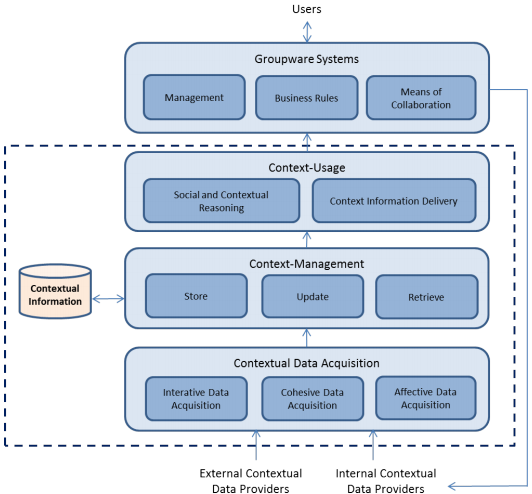
\includegraphics[scale=0.6]{arch}
  \caption{Arquitectura para soportar colaboraci\'on en groupware conscientes del contexto \cite{montane2013context}}
\end{figure}

Para que una arquitectura sea consciente del contexto debe de cumplir con los siguientes requerimientos\cite{dey1999architecture}:
\begin{itemize}
\item Permitir a las aplicaciones acceder a informaci\'on contextual desde m\'aquinas distribuidas en el de la misma forma en que acceden a la entrada del usuario en una m\'aquina local.
\item Soportar la ejecuci\'on de diferentes plataformas y el uso de diferentes lenguajes de programaci\'on.
\item Soportar la interpretaci\'on de informaci\'on contextual.
\item Soportar la agregaci\'on de informaci\'on contextual
\item Soportar independencia y persistencia de widgets contextuales
\item Soportar el almacenamiento del historial de contexto
\end{itemize}

Tambi\'en para el soporte de consciencia contextual, Elg Ghayam \cite{el2011distributed} menciona 2 requerimientos que se deben de cumplir: la formalizaci\'on de contexto, para delimitar los datos contextuales y facilitar la distinci\'on de par\'ametros de contexto, una categorizaci\'on de datos contextuales es requerida, m\'as aun, para reducir la complejidad de su manutenci\'on, una representaci\'on formal tambi\'en es necesaria. El otro punto son reglas de adaptaci\'on: la adaptaci\'on de contexto debe de ser vista como un conjunto de reglas que controlan y anticipan el cambio de contexto que puede ocurrir en el ambiente, por lo tanto, en la construcci\'on de reglas de adaptaci\'on, el n\'umero de par\'ametros contextuales es grande y as\'i, no es evidente que no se pueden enumerar todas las posibles situaciones que van a ocurrir. Por lo anterior, un m\'etodo para construir reglas de adaptaci\'on es requerido, que pueda manejar la diversidad de posibles situaciones que se construyen en base de esos par\'ametros contextuales.

Para poder mejorar la colaboraci\'on de los usuarios, la arquitectura debe de permitir que el groupware pueda adaptarse al contexto, y de acuerdo a Abowd\cite{abowd1999towards} hay 3 tipos de adaptaci\'on:
\begin{itemize}
\item  Presentaci\'on de informaci\'on y servicios al usuario. Se refiere a la t\'ecnica de interacci\'on que muestra una lista de objetos o lugares cuyos elementos m\'as importantes son resaltados de acuerdo al contexto actual del usuario.
\item Ejecuci\'on autom\'atica de un servicio. En este caso un servicio es autom\'aticamente lanzado si la combinaci\'on correcta de condiciones es dada.
\item Aumento de la informaci\'on. Informaci\'on contextual puede servir para entender mejor el ambiente colaborativo.
\end{itemize}

Muchas arquitecturas se han propuesto para poder soportar sistemas conscientes del contexto, la siguiente tabla hace una comparaci\'on de los elementos y capas de algunas arquitecturas conscientes del contexto, entre las cuales se encuentran la arquitectura base para el presente trabajo que usa un modelo contextual colaborativo clasificado en tres categor\'ias: elementos cohesivos, elementos interactivos y elementos afectivos. La arquitectura de Dey\cite{dey1999architecture}  usa widgets para la captura de datos contextuales y servicios de agregaci\'on de contexto as\'i como servicios de distribuci\'on y razonamiento contextual. En el marco de trabajo de Kamoun \cite{kamoun2012fadyrcos}  se reconfiguran servicios para adaptarlos a situaciones que cambian din\'amicamente. Decouchant \cite{decouchant2013adapting} divide su arquitectura en tres capas: la capa de espacio de trabajo, la de adaptaci\'on y la de detecci\'on de informaci\'on contextual. Guerman  \cite{guermah2013ontology} que propone una arquitectura orientada a sistemas de aprendizaje electr\'onico. En la figura \ref{cmp:fig} se comparan algunos elementos que poseen dichas arquitecturas, entre ellos se encuentran la presencia de capas como adquisici\'on, manejo y distribuci\'on de datos contextuales, persistencia de datos y su reuso, apoyo con v\'ias de comunicaci\'on, el uso de widgets como comunicadores entre el sistema y la arquitectura, manejo de sesiones, esquemas conceptuales de colaboraci\'on, agregaci\'on de datos y la representaci\'on de espacios de trabajo como parte de la arquitectura.

\begin{figure}[h!]
  \centering
    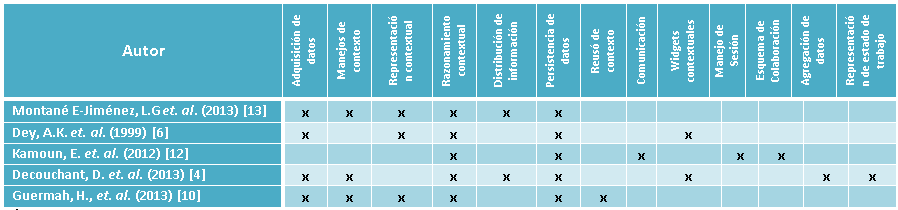
\includegraphics[scale=0.7]{images/comparaciones.png}
  \caption{Comparaci\'on de arquitecturas que soportan consciencia del contexto\cite{montane2013context}\cite{dey1999architecture}\cite{kamoun2012fadyrcos}\cite{decouchant2013adapting}\cite{guermah2013ontology}}
  \label{cmp:fig}
\end{figure}
